\documentclass[english,xcolor=svgnames]{beamer}


\usepackage{mathptmx}
\usepackage[OT1]{fontenc}
% \usepackage[latin9]{inputenc}
\usepackage{amsmath}
\usepackage{amssymb}
\usepackage{amsthm}
\usepackage{mathrsfs}
\usepackage{amsfonts}
\usepackage{eurosym}
\usepackage{bm}

\usepackage{booktabs}
\usepackage{tabularx}
\usepackage{subcaption}
\usepackage[makeroom,thicklines]{cancel}

\usepackage{multirow}
\usepackage{rotating}
\usepackage{array}
\usepackage{float}



\makeatletter

 \newcommand\makebeamertitle{\frame{\maketitle}}%
 \AtBeginDocument{
   \let\origtableofcontents=\tableofcontents
 \def\tableofcontents{\@ifnextchar[{\origtableofcontents}{\gobbletableofcontents}}
   \def\gobbletableofcontents#1{\origtableofcontents}
 }
 
 \usetheme{Boadilla}
\setbeamertemplate{footline}[frame number]{}
\usefonttheme{structuresmallcapsserif}
\setbeamercolor{title}{fg=blue}
\setbeamercolor{frametitle}{fg=blue}
\setbeamercolor{caption name}{fg=blue}
\setbeamercovered{transparent}


\beamertemplatenavigationsymbolsempty

\usepackage{booktabs}
\usepackage{tabularx}
\renewcommand{\tabularxcolumn}[1]{>{\centering\arraybackslash}m{#1}}
%\newcolumntype{L}{>{\centering}X}
%\newcolumntype{H}{>{\lrbox0}c<{\endlrbox}@{}}

%\let\estinput=\input
%\newcommand{\estwide}[3]{
%          \vspace{.75ex}{
%               \begin{tabularx}
%               {\textwidth}{@{\hskip\tabcolsep\extracolsep\fill}l*{#2}{#3}}
%               \toprule
%               \estinput{#1}
%               \bottomrule
%               \addlinespace[.75ex]
%               \end{tabularx}
%               }
%          }
%
%		\newcommand{\figtext}[1]{
%		     %\vspace{-1.9ex}
%		     \captionsetup{justification=justified,font=footnotesize}
%		     \caption*{\hspace{6pt}\hangindent=1.5em #1}
%		     }
%		\newcommand{\fignote}[1]{\figtext{\emph{Note:~}~#1}}
%
\usepackage{collcell}
%\makeatother
% \newcolumntype{G}{>{\collectcell\@gobble}c<{\endcollectcell}@{}}
% \makeatother
% \def\eatcell#1\unskip{}
% \newcolumntype{E}{>{\eatcell}c@{}}
%\usepackage{tabulary}
%\usepackage{multirow}
%\usepackage{dcolumn}
%\usepackage{pdflscape}
%\usepackage{pdfpages}
% \usepackage{epsfig}
% \usepackage{epstopdf}
% \usepackage{eso-pic}
\usepackage{graphicx}
%\usepackage{arydshln}
\usepackage[compatibility=false,font={sc,rm,color=blue},justification=centering,labelformat=empty, textfont=Large, margin=2pt]{caption}
\captionsetup[figure]{belowskip=0pt}

\newcommand{\rot}[2]{\rule{1em}{0pt}%
\makebox[0cm][c]{\rotatebox{#1}{\ #2}}}

\usepackage{siunitx} %For aligning decimals
\sisetup{ detect-mode, 
          group-digits            = false ,
          input-signs             = ,
          input-symbols           = ()[]-+* ,
          input-open-uncertainty  = ,
          input-close-uncertainty = ,
          table-align-text-post   = false, 
          table-number-alignment = center
}
\selectcolormodel{cmyk}
\usepackage{color,soul}
\usepackage{colortbl}
\usepackage{tikz}
\usetikzlibrary{matrix,shapes,arrows,intersections,calc}
\usepackage{verbatim}
\setbeamercovered{invisible}
\setbeamercolor{math text displayed}{fg=blue}
\setbeamercolor{math text inlined}{fg=blue}

%\let\olditem\item
%\renewcommand{\item}{\setlength{\itemsep}{\fill}\olditem}
\AtBeginDocument{\setlength\belowdisplayskip{0pt}}


\usepackage[english]{babel}
\usepackage{booktabs}
\usepackage{tablefootnote}
\usepackage{calc,hhline,ifthen,lscape} 

%\usepackage{enumitem}
%\let\olditem\item
%\renewcommand{\item}{\setlength{\itemsep}{\fill}\olditem}

% new math commands
\newcommand{\E}{\mathbb{E}}

\newcommand{\sym}[1]{\rlap{$#1$}} %For sym in STATA tables

\setbeamertemplate{frametitle}[default][center]

% \makeglossaries
% 
% \usepackage{pgfpages}
% \pgfpagesuselayout{resize to}[a4paper, landscape, border shrink=5mm]
\usepackage[absolute,overlay]{textpos}

\usepackage{epstopdf}


%\setlength{\itemsep}{\fill}



% ===========================================================
% ===========================================================
% ===========================================================
% Improves spacing of itemize and enumerate environment

\makeatletter
\renewcommand{\itemize}[1][]{%
  \beamer@ifempty{#1}{}{\def\beamer@defaultospec{#1}}%
  \ifnum \@itemdepth >2\relax\@toodeep\else
    \advance\@itemdepth\@ne
    \beamer@computepref\@itemdepth% sets \beameritemnestingprefix
    \usebeamerfont{itemize/enumerate \beameritemnestingprefix body}%
    \usebeamercolor[fg]{itemize/enumerate \beameritemnestingprefix body}%
    \usebeamertemplate{itemize/enumerate \beameritemnestingprefix body begin}%
    \list
      {\usebeamertemplate{itemize \beameritemnestingprefix item}}
      {\def\makelabel##1{%
          {%
            \hss\llap{{%
                \usebeamerfont*{itemize \beameritemnestingprefix item}%
                \usebeamercolor[fg]{itemize \beameritemnestingprefix item}##1}}%
          }%
        }%
      }
  \fi%
  \setlength\itemsep{\fill}
    \ifnum \@itemdepth >1
        \vfill
    \fi%  
  \beamer@cramped%
  \raggedright%
  \beamer@firstlineitemizeunskip%
}

\def\enditemize{\ifhmode\unskip\fi\endlist%
  \usebeamertemplate{itemize/enumerate \beameritemnestingprefix body end}
  \ifnum \@itemdepth >1
        \vfil
  \fi%  
  }
\makeatother


\makeatletter
\def\enumerate{%
	\ifnum\@enumdepth>2\relax\@toodeep
	\else%
	\advance\@enumdepth\@ne%
	\edef\@enumctr{enum\romannumeral\the\@enumdepth}%
	\advance\@itemdepth\@ne%
	\fi%
	\beamer@computepref\@enumdepth% sets \beameritemnestingprefix
	\edef\beamer@enumtempl{enumerate \beameritemnestingprefix item}%
	\@ifnextchar[{\beamer@@enum@}{\beamer@enum@}}
\def\beamer@@enum@[{\@ifnextchar<{\beamer@enumdefault[}{\beamer@@@enum@[}}
\def\beamer@enumdefault[#1]{\def\beamer@defaultospec{#1}%
	\@ifnextchar[{\beamer@@@enum@}{\beamer@enum@}}
\def\beamer@@@enum@[#1]{% partly copied from enumerate.sty
	\@enLab{}\let\@enThe\@enQmark
	\@enloop#1\@enum@
	\ifx\@enThe\@enQmark\@warning{The counter will not be printed.%
		^^J\space\@spaces\@spaces\@spaces The label is: \the\@enLab}\fi
	\def\insertenumlabel{\the\@enLab}
	\def\beamer@enumtempl{enumerate mini template}%
	\expandafter\let\csname the\@enumctr\endcsname\@enThe
	\csname c@\@enumctr\endcsname7
	\expandafter\settowidth
	\csname leftmargin\romannumeral\@enumdepth\endcsname
	{\the\@enLab\hspace{\labelsep}}%
	\beamer@enum@}
\def\beamer@enum@{%
	\beamer@computepref\@itemdepth% sets \beameritemnestingprefix
	\usebeamerfont{itemize/enumerate \beameritemnestingprefix body}%
	\usebeamercolor[fg]{itemize/enumerate \beameritemnestingprefix body}%
	\usebeamertemplate{itemize/enumerate \beameritemnestingprefix body begin}%
	\expandafter
	\list
	{\usebeamertemplate{\beamer@enumtempl}}
	{\usecounter\@enumctr%
		\def\makelabel##1{{\hss\llap{{%
						\usebeamerfont*{enumerate \beameritemnestingprefix item}%
						\usebeamercolor[fg]{enumerate \beameritemnestingprefix item}##1}}}}}%
	\setlength\itemsep{\fill}
	\ifnum \@itemdepth >1
	\vfill
	\fi%  
	\beamer@cramped%
	\raggedright%
	\beamer@firstlineitemizeunskip%
}
\def\endenumerate{\ifhmode\unskip\fi\endlist%
	\usebeamertemplate{itemize/enumerate \beameritemnestingprefix body end}
	\ifnum \@itemdepth >1
	\vfil
	\fi%  
}
\makeatother

% ===========================================================
% ===========================================================
% ===========================================================


%\usepackage[colorlinks=true]{hyperref}

\hypersetup{colorlinks = true,linkcolor = blue, bookmarksopen=true, bookmarksopenlevel=1}

%\hypersetup{bookmarksopen=true, bookmarksopenlevel=1}



\begin{document}

\title{Regional Aggregation II \& Household Aggregation}
\vspace{1cm}
\author[shortname]{
\begin{tabular}{cc}
Juan Herre\~{n}o & Johannes Wieland \\ 
\end{tabular}\\
}



\date{UCSD, Spring \the\year}

\setbeamertemplate{footline}{}
\makebeamertitle
\setbeamertemplate{footline}[frame number]{}

\addtocounter{framenumber}{-1}

%%%%%%%%%%%%%%%%%%%%%%%%%%%%%%%%%%%%%%%%%%%%%%%%%%
\AtBeginSection[]{
\setbeamertemplate{footline}{}
  \frame<beamer>{ 

    \frametitle{Outline}   

    \tableofcontents[currentsection,hideallsubsections] 
  }
\setbeamertemplate{footline}[frame number]{}
\addtocounter{framenumber}{-1}
}

\AtBeginSubsection[]{
\setbeamertemplate{footline}{}
  \frame<beamer>{ 

    \frametitle{Outline}   

    \tableofcontents[currentsection,currentsubsection] 
  }
  \setbeamertemplate{footline}[frame number]{}
  \addtocounter{framenumber}{-1}
}



\setbeamertemplate{footline}{}
\begin{frame}
\frametitle{Outline}   
\tableofcontents[hideallsubsections] 
\end{frame}
\addtocounter{framenumber}{-1}
\setbeamertemplate{footline}[frame number]{}


%%%%%%%%%%%%%%%%%%%%%%%%%%%%%%%%%%%%%%%%%%%%%%%%%%
\section{Introduction}
%%%%%%%%%%%%%%%%%%%%%%%%%%%%%%%%%%%%%%%%%%%%%%%%%%

\begin{frame}
\frametitle[alignment=center]{Monetary Transmission Mechanism}
\begin{itemize}
	\item Intertemporal substitution (changes in the real interest rate affect C and I).
	\item Credit channel: monetary changes affect spreads, ability of banks to make loans, etc. (Jim\'{e}nez, Ongena, Peydr\'{o}, and Saurina, AER 2012)
	\item Relaxing liquidity constraints for some households by raising income (Cloyne, Ferreira, and Surico, ReStud 2020).
	\item Redistribute income to high MPC consumers (Hausman, Rhode, and Wieland, AER 2019).
	\item Increases real money balances (Chodorow-Reich, Gopinath, Mishra, Narayanan, QJE 2019).
\end{itemize}
\end{frame}


%%%%%%%%%%%%%%%%%%%%%%%%%%%%%%%%%%%%%%%%%%%%%%%%%%
\section{Hausman, Rhode, and Wieland (2019, AER)}
%%%%%%%%%%%%%%%%%%%%%%%%%%%%%%%%%%%%%%%%%%%%%%%%%%

\begin{frame}
\frametitle[alignment=center]{Recovery from the Great Depression}
\centering
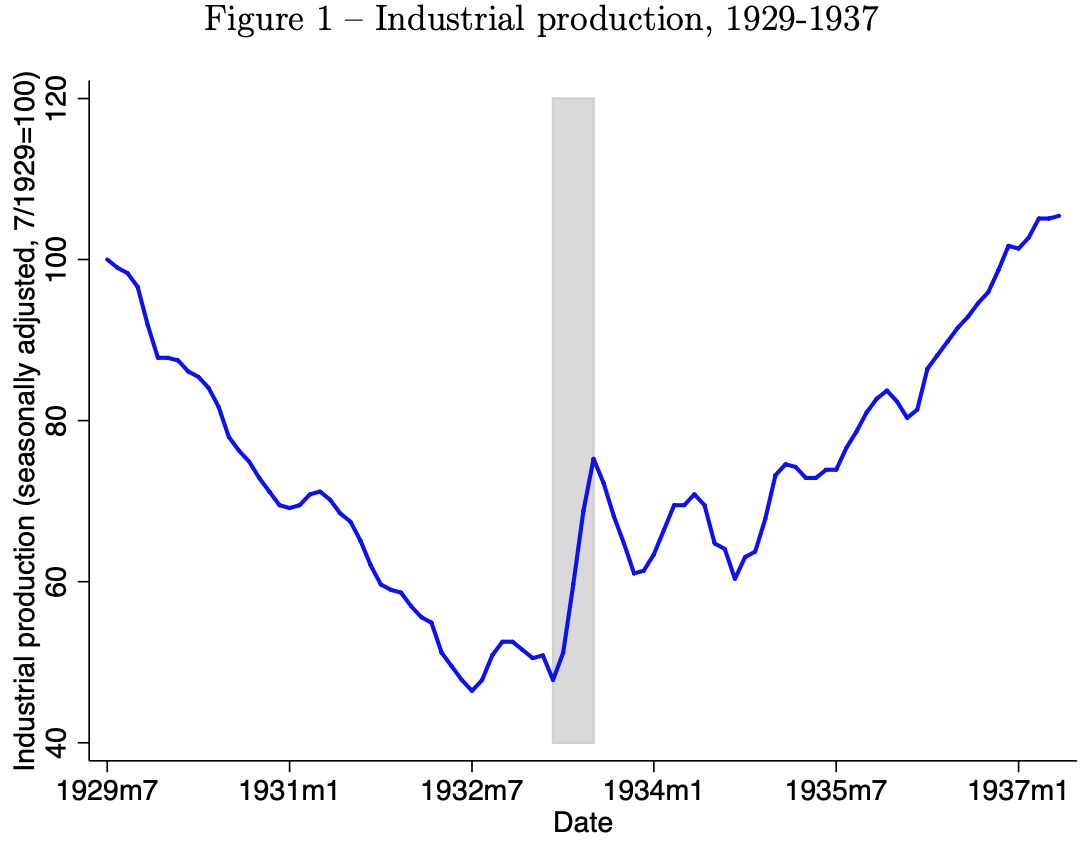
\includegraphics[scale=0.5]{figures/HRWFIG1.png}
\end{frame}

\begin{frame}
\frametitle[alignment=center]{Large Devaluation from Leaving Gold Standard}
\centering
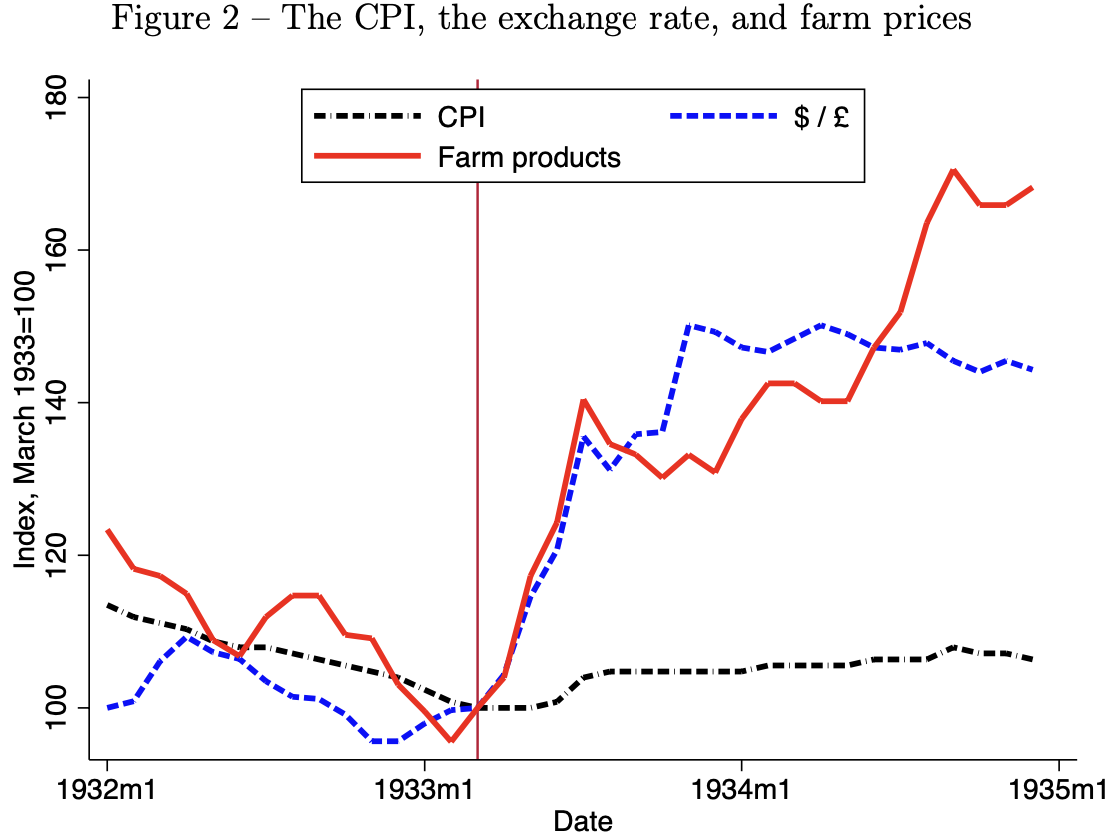
\includegraphics[scale=0.5]{figures/HRWFIG2.png}
\end{frame}

\begin{frame}
\frametitle[alignment=center]{Tradable Prices Rose}
\centering
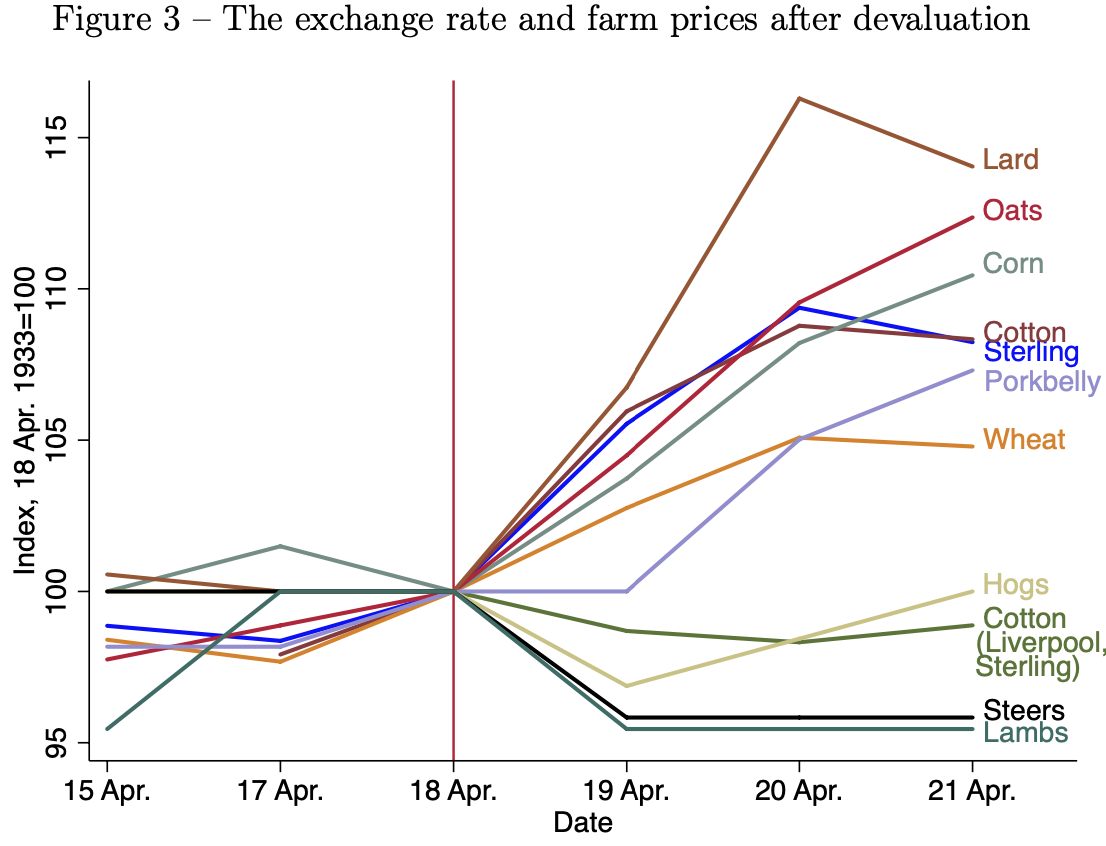
\includegraphics[scale=0.5]{figures/HRWFIG3.png}
\end{frame}

\begin{frame}
\frametitle[alignment=center]{Farm Incomes Rose}
\centering
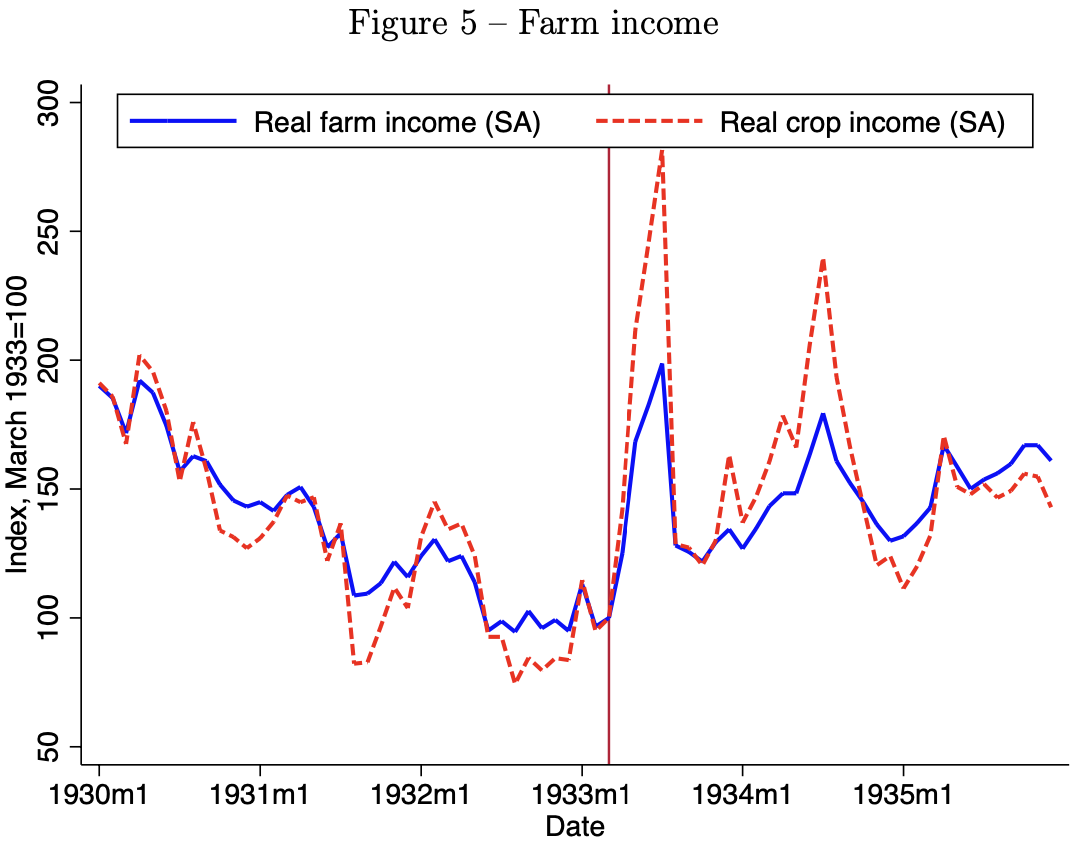
\includegraphics[scale=0.5]{figures/HRWFIG5.png}
\end{frame}


\begin{frame}
\frametitle[alignment=center]{Specification}
\begin{itemize}
	\item Cross-sectional regression of the form:
	\begin{align*}
		\%\Delta \text{Auto sales}_{i,\text{Spring 1933}} = \beta_0 + \beta_1 \text{Agricultural exposure}_i + \gamma'X_i+\epsilon_i
	\end{align*}
	\item What is the identifying assumption?
	\item Comments? Concerns?
\end{itemize}
\end{frame}

\begin{frame}
\frametitle[alignment=center]{Test for Pre-Trends}
\centering
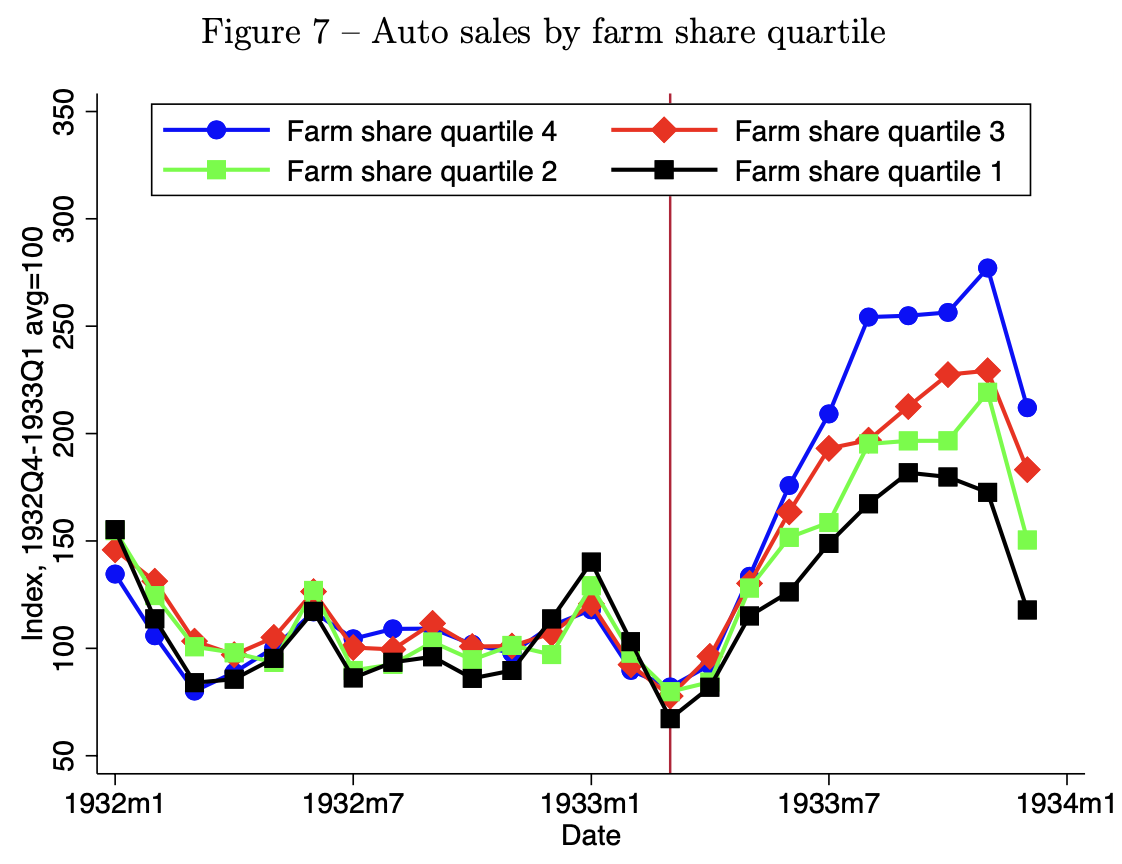
\includegraphics[scale=0.5]{figures/HRWFIG7.png}
\end{frame}

\begin{frame}
\frametitle[alignment=center]{County-level Analysis}
\centering
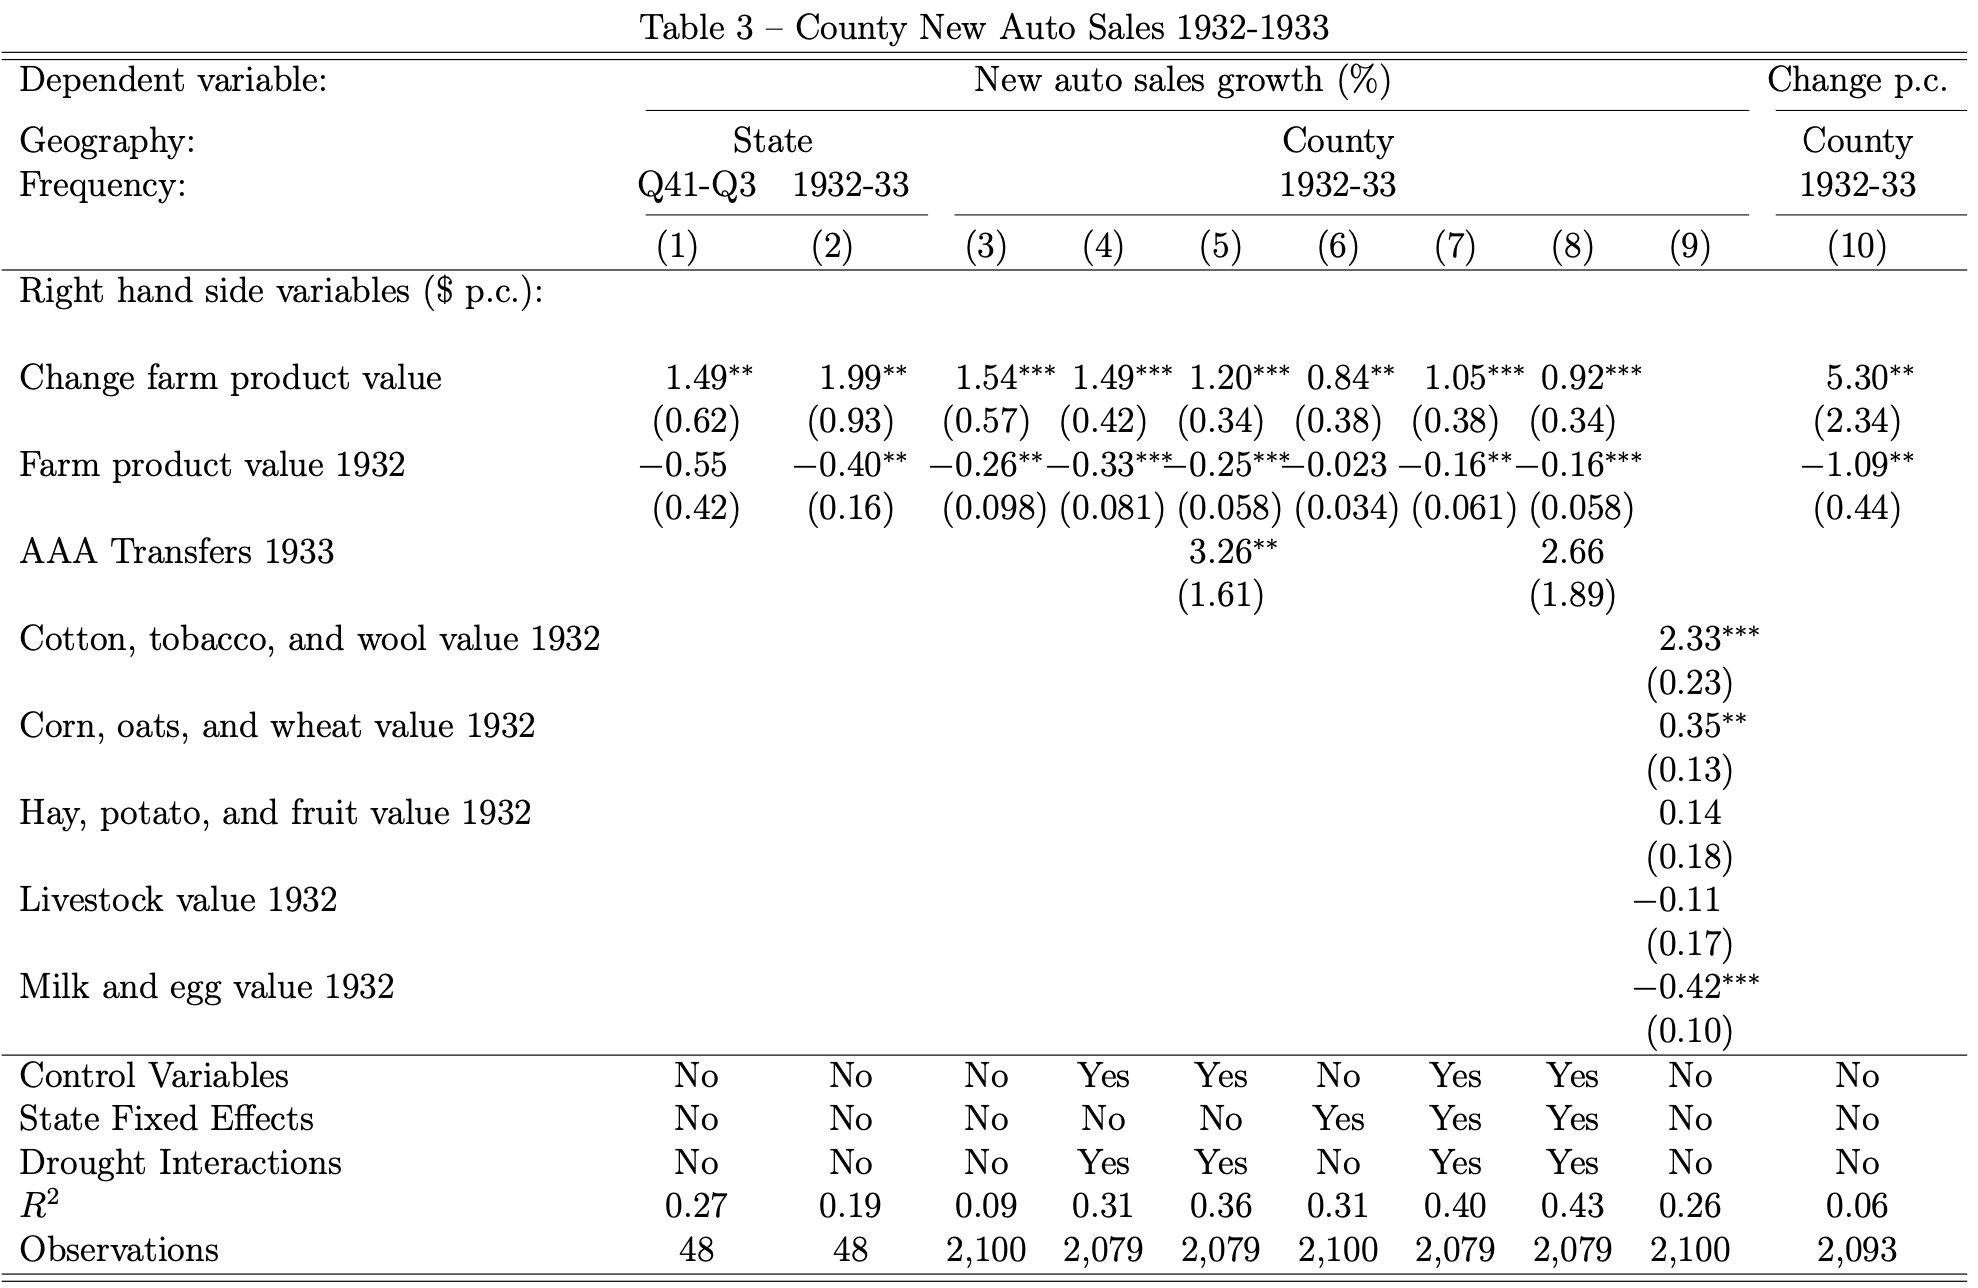
\includegraphics[scale=0.4]{figures/HRWTAB3.png}
\end{frame}

\begin{frame}
\frametitle[alignment=center]{Convincing?}

\end{frame}

\begin{frame}
\frametitle[alignment=center]{Aggregation Effects?}
\begin{itemize}
	\item Evidence is about \emph{relative} changes in consumption expenditure.
	\item Three mechanisms by which it can be expansionary overall:
	\begin{enumerate}
		\item Redistribution to higher-MPC households.
		\item Improves bank health.
		\item Raises inflation expectations.
	\end{enumerate}
\end{itemize}
\end{frame}

\begin{frame}
\frametitle[alignment=center]{Testing for Differential MPCs}
\begin{itemize}
	\item Cross-sectional regression of the form:
	\begin{align*}
		\%\Delta &\text{Auto sales}_{i,\text{Spring 1933}} =\\
		&  \beta_0 + \beta_1 \Delta\text{farm product value}_i \times \% \text{farms mortgaged} + \\ 
		&+ \beta_2 \text{farm product value}_i \times \% \text{farms mortgaged} \\
		&+ \beta_3 \Delta\text{farm product value}_i  +\beta_4 \% \text{farms mortgaged} \\
		& + \beta_5 \Delta\text{farm product value}_i  + \gamma'X_i+\epsilon_i
	\end{align*}
	\item What is the identifying assumption?
	\item Comments? Concerns?
\end{itemize}
\end{frame}

\begin{frame}
\frametitle[alignment=center]{Debt-Interaction Positiv}
\centering
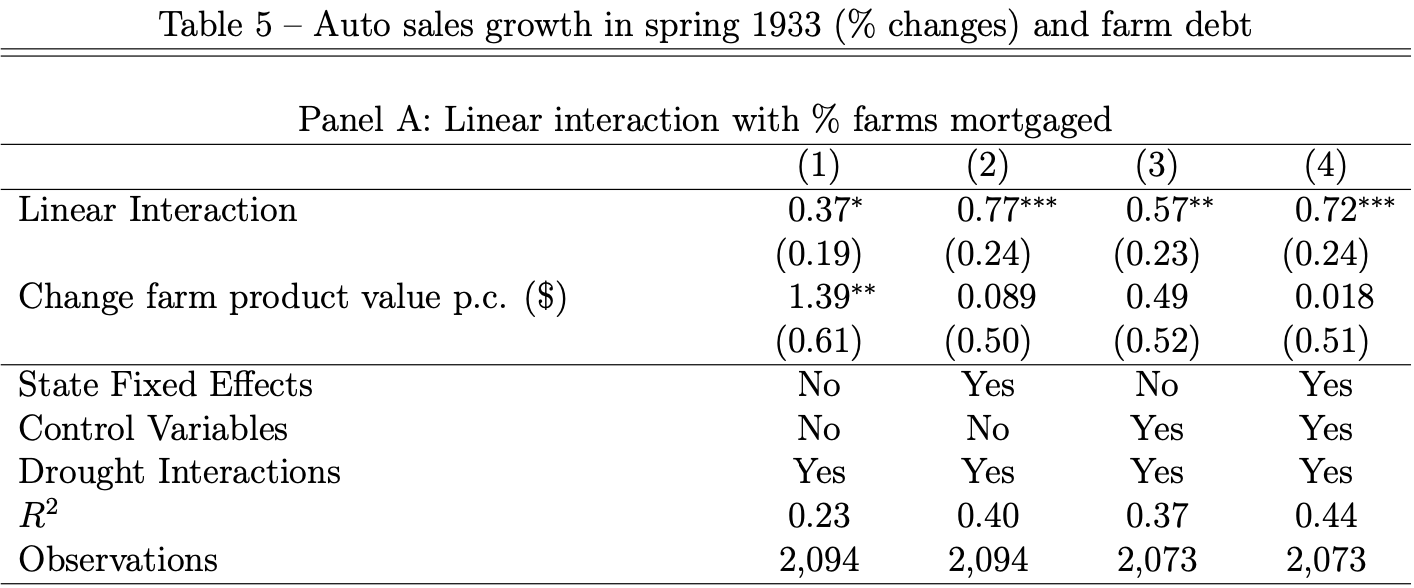
\includegraphics[scale=0.4]{figures/HRWTAB5a.png}
\end{frame}

\begin{frame}
\frametitle[alignment=center]{Differential Deposit Growth}
\centering
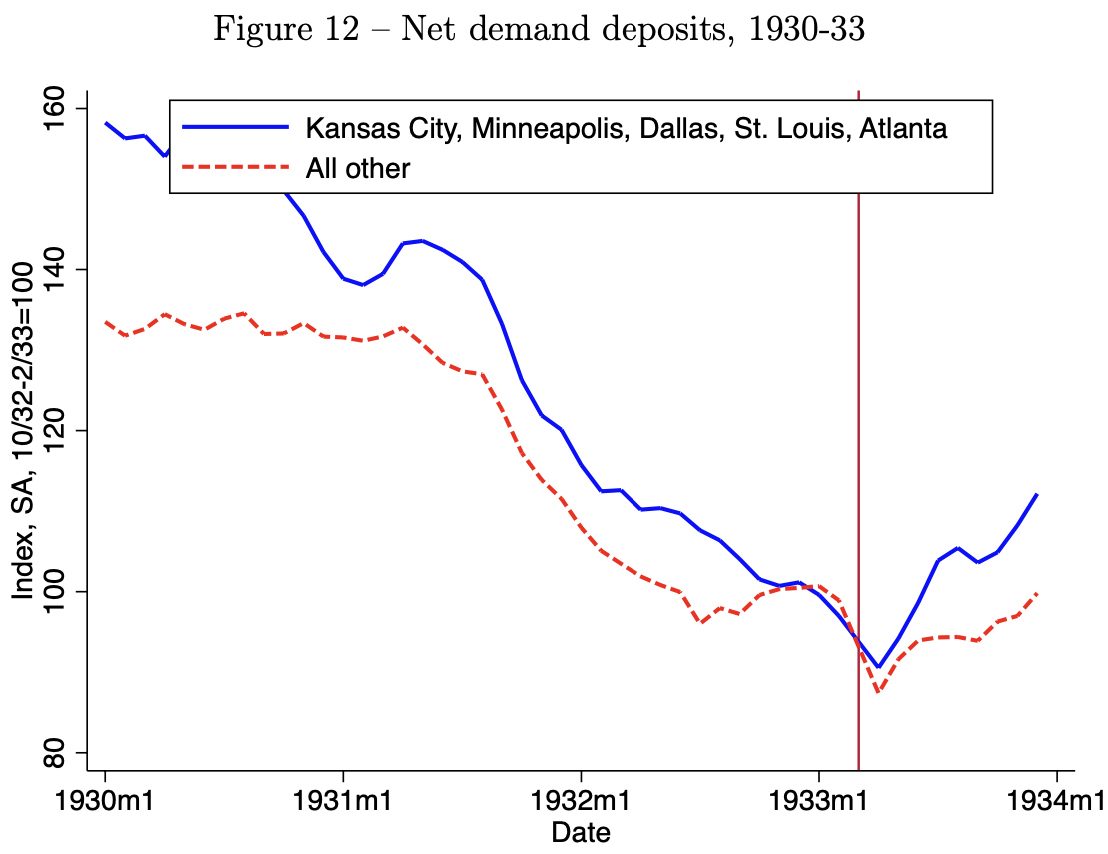
\includegraphics[scale=0.5]{figures/HRWFIG12.png}
\end{frame}

\begin{frame}
\frametitle[alignment=center]{Inflation Expectations?}
\centering

\includegraphics[scale=0.5]{figures/HRWFIG14b.png}
\end{frame}

\begin{frame}
\frametitle{Aggregation}

\begin{itemize}
\item Simple framework to examine how cross-sectional estimates map to the aggregate economy.
\item Model has heterogeneity on the following three dimensions:
\begin{itemize}
	\item Income from farming, labor, or pricing power.
	\item Permanent income vs hand-to-mouth.
	\item Farm vs urban area.
\end{itemize}
\item Simplifications:
\begin{itemize}
	\item Model essentially static.
	\item Exogenous relative price movements.
\end{itemize}
\item Who studied the appendix?
\end{itemize}

\end{frame}

\begin{frame}
\frametitle{Key result}
\vspace{-0.8cm}
\begin{align*}
	\% \Delta \text{Cars} &= \underbrace{\beta \times
                         \phi^{f}}_{\substack{\text{``naive''} \\
  \text{extrapolation}}} \times  \underbrace{\frac{\text{Farm
  area income per capita}}{\text{National income per
  capita}}}_{\text{Relative income p.c.}} \\
  & \times  \underbrace{\left( 1-\xi\frac{\theta^{w}}{\theta^{f}} \right)}_{\substack{\text{Redistribution from } \\ \text{high-MPC consumers}}} \times \underbrace{\mu_{t}}_{\substack{\text{Aggregate}\\ \text{spending}\\ \text{multiplier}}} \\
  &\qquad  + \underbrace{-\sigma  d\ln (1+r_t)}_{\text{Intertemporal Substitution}}
\end{align*}
\begin{itemize}
	\item Comments? Concerns?
\end{itemize}

\end{frame}

\begin{frame}
\frametitle[alignment=center]{Debt-Interaction Positive}
\centering
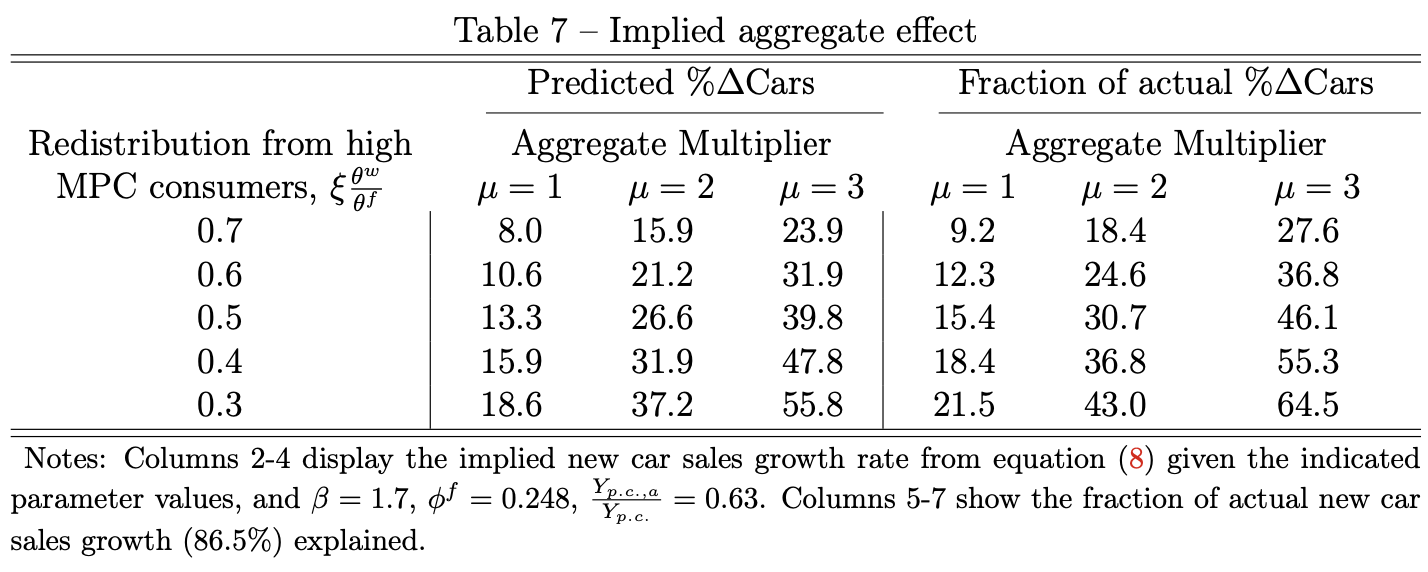
\includegraphics[scale=0.4]{figures/HRWTAB7.png}
\begin{itemize}
	\item Thoughts? Comments?
\end{itemize}
\end{frame}

%\begin{frame}
%\frametitle{Preferences}
%
%\begin{itemize}
%	\item Three agents: farmers $f$, workers $w$ and capitalists $c$.
%	\item Population shares: $\phi^{f}$, $\phi^{w}$, and $1-\phi^{f}-\phi^{w}$.
%	\item Utility function:
%	\begin{align*}
%	\sum_{t=1}^{\infty} \beta^{t-1} \left[\ln c_{t}+\psi \ln d_{t}\right],
%\end{align*}
%\item One-period non-contingent loans the only asset.
%\item Borrowing limit:
%\begin{align*}
%	a_{t}^{x}\ge s^{x}\bar{a},\qquad\qquad x\in\{f,w,c\} \\
%\end{align*}
%$s^x$ is steady-state income share of agents $x$.
%\end{itemize}
%
%\end{frame}


%\begin{frame}
%\frametitle{Technologies and prices}
%
%\begin{itemize}
%	\item Production function for bread and cars
%	\begin{align*}
%		C_{t} &= \min\{\alpha^{-1} X_{t},(1-\alpha)^{-1}L_{c,t}\} \\
%		D_{t} &= L_{d,t}
%\end{align*}
%	\item Potential farm output $\bar{X}$ and labor supply $\bar{L}$.
%	\item Bread and car prices fixed at 1.
%	\item Real wage fixed. % at $w=m^{-1}<1$.
%	\item Exogenous real farm price $p_{x,t}$.
%	\item Interest rate rule ensures full employment s.t. ZLB constraint.
%\end{itemize}
%
%\end{frame}
%
%
%\begin{frame}[label=fix-price]
%\frametitle{Fixed prices assumption}
%
%3 reasons
%\begin{enumerate}
%\item Simplifies the model.
%\item Consistent with some evidence. 
%\begin{itemize}
%\item CPI unchanged March to May 1933.
%\item Retail price of bread unchanged March to June 1933 despite 49\%
%  increase in wheat price. \vfill
%%\item But retail lard prices up 21\% March to June 1933. (Wholesale up
%%  38\%.) \vfill
%\end{itemize}
%\item No obvious net bias to model.
%\begin{itemize}
%\item Rules out negative effect on workers from higher farm
%  prices.
%\item Rules out positive effect on aggregate economy from higher expected inflation caused
%  by higher farm prices. \hyperlink{latimes}{\beamergotobutton{Article}}
%\end{itemize}
%\end{enumerate}
%\end{frame}
%
%
%\begin{frame}
%\frametitle{Interest-rate rule and timing}
%
%Interest rate rule: output equal to potential unless ZLB
%          binds.
%
%\begin{itemize}
%	\item $t=1$ Farm prices such that:\vfill
%\begin{itemize}
%	%	\item $p_{x,1}<w-\frac{1+\psi}{\alpha}(1-m^{-1})\frac{-\beta\kappa_1\bar{a}}{\bar{Y}-\beta\kappa_1\bar{a}}$
%		%\item[$\Rightarrow$] ZLB binding.
%		%\item[$\Rightarrow$] Borrowing constraints for
%                %farmers and workers bind.\vfill
%	\item Borrowing constraints for farmers and workers bind. Their MPC=1.        
%        \item  ZLB binding and recession.
%          \vfill
%	\end{itemize}	
%	\item $t\ge 2$ Farm prices such that:\vfill
%	\begin{itemize}
%	%	\item $p_{x,t}=w$
%	%	\item[$\Rightarrow$] ZLB not binding.
%	%	\item[$\Rightarrow$] All borrowing constraints
%              %    slack.\vfill
%               \item All borrowing constraints slack.
%                \item ZLB not binding and full employment.\vfill	
%	\end{itemize}
%	\item Spring 1933: in $t=1$, increase farm price $p_{x,t}$.
%\end{itemize}
%\end{frame}
%
%
%\begin{frame}
%\frametitle{Solution: $t=1$}
%\begin{itemize}
%	\item Aggregate output: Keynesian cross
%	\begin{align*}
%		Y_{1}=\frac{1}{s_{1}^{c}(1-mpc^{c})}\left[-(1-s^{c})\bar{a}+\beta^{-1}(1-mpc^{c})s^{c} \bar{Y}\right].
%	\end{align*}
%	\vspace{0.2cm}
%	\begin{itemize}
%		\item Weighted mpc: $s_{1}^{c}(1-mpc^{c})=1-s_1^{c}\times mpc^{c}-(1-s_1^{c})\times 1$
%		\item Autonomous consumption: $-(1-s^{c})\bar{a}+\beta^{-1}(1-mpc^{c})s^{c} \bar{Y}$ \vfill
%	\end{itemize}
%	\item Redistribution channel:
%	\begin{align*}
%	\frac{dY_{1}/Y_{1}}{dp_{x,1}/p_{x,1}}&=\frac{s_{1}^{f}}{s_{1}^{c}}=\frac{\mbox{farm
%                                               share of
%                                               income}}{\mbox{capitalist
%                                               share of income}}>0
%\end{align*}
%\end{itemize}
%\end{frame}
%
%
%\begin{frame}
%\frametitle{Cross-section: $t=1$}
%\begin{itemize}
%\item Two areas: agriculture $a$, manufacturing $m$.
%\item Farmers, bakers, capitalists live in $a$; bakers, laborers, capitalists live in $m$.
%\item $c$ non-traded (bread), $d$ traded (cars).
%\item ``Regression'':
%\begin{align*}
%	\frac{d D_{i,t}}{D_{i,t}}= \alpha + \beta \frac{\phi_i^{f}}{\phi_{i}},\qquad i=a,m
%\end{align*}
%\item Result:
%\begin{align*}
%	 \beta \phi^{f}&\le \underbrace{\frac{1}{1-s^{b}}}_{\text{Local multiplier}} \underbrace{\frac{d p_{x,t}}{p_{x,t}}s_{1}^{f}}_{\Delta\text{farm income}} \underbrace{\left(\frac{Y_{p.c.,a,t} }{ Y_{p.c.,t} }\right)^{-1}}_{\text{Rel p.c. income}} 
%\end{align*}
%%\item Income:
%%\begin{align*}
%%		y_{a,t}^{f} &=  s_{t}^{f}Y_{t},\qquad &y_{a,t}^{b} &= s^{b}s_{a,t}Y_{t},\qquad &y_{m,t}^{b} &= s^{b}s_{m,t}Y_{t},\\ y_{m,t}^{l} &=  s^{l}Y_{t}, \qquad &y_{a,t}^{c} &=  s_a s_{t}^{c}Y_{t}, \qquad & y_{m,t}^{c} &=  s_m s_{t}^{c}Y_{t}
%%	\end{align*}
%%\item Total car expenditure:
%%\begin{align*}
%%		D_{a,1}&=\frac{\psi}{1+\psi}s_{a,1}Y_{1};\qquad &
%%		D_{m,1}&=\frac{\psi}{1+\psi}s_{m,1}Y_{1}.
%%	\end{align*}
%\end{itemize}
%
%\end{frame}
%
%
%\begin{frame}
%\frametitle{Cross-section: $t=1$}
%
%\begin{align*}
%	\frac{d Y_t}{Y_{t}} \ge   \underbrace{\beta}_{\text{X-section}} \times \underbrace{\phi^{f}}_{\text{farm population share}} \times \underbrace{\frac{Y_{p.c.,a,t}}{Y_{p.c.,t}}}_{\text{Rel. income p.c. farm states}}.
%\end{align*}
%%$\beta \approx 1.7 $, $\phi^{f}=25\%$, $\phi^{f}=25\%$ $\implies$ increase in farm
%%  prices explains 30\% (or more) of the auto sales/production increase.
%\vspace{0.2cm}
%\begin{itemize}
%\item Local multiplier $<$ aggregate multiplier $\Rightarrow$ Inequality.\vfill
%\begin{itemize}
%\item Expenditure leakage to non-farm area.
%\item At ZLB, no monetary policy response to lower aggregate relative to
%  local multiplier.
% \item Sticky prices $\Rightarrow$ no terms-of-trade response.\vfill
% \end{itemize}	
% \item Result specific to circumstances in Spring 1933.
%\end{itemize}
%\end{frame}


%%%%%%%%%%%%%%%%%%%%%%%%%%%%%%%%%%%%%%%%%%%%%%%%%%
\section{Cloyne, Ferreira, and Surico (2020, ReStud)}
%%%%%%%%%%%%%%%%%%%%%%%%%%%%%%%%%%%%%%%%%%%%%%%%%%

\begin{frame}
\frametitle[alignment=center]{Monetary Transmission Mechanism}
\begin{itemize}
	\item x
\end{itemize}
\end{frame}


%%%%%%%%%%%%%%%%%%%%%%%%%%%%%%%%%%%%%%%%%%%%%%%%%%
\section{Parker, Souleles, Johnson, and McClelland (2013, AER)}
%%%%%%%%%%%%%%%%%%%%%%%%%%%%%%%%%%%%%%%%%%%%%%%%%%

\begin{frame}
\frametitle[alignment=center]{Monetary Transmission Mechanism}
\begin{itemize}
	\item x
\end{itemize}
\end{frame}


%%%%%%%%%%%%%%%%%%%%%%%%%%%%%%%%%%%%%%%%%%%%%%%%%%
\section{Borusyak, Jaravel, and Spiess (2022, WP)}
%%%%%%%%%%%%%%%%%%%%%%%%%%%%%%%%%%%%%%%%%%%%%%%%%%

\begin{frame}
\frametitle[alignment=center]{Monetary Transmission Mechanism}
\begin{itemize}
	\item x
\end{itemize}
\end{frame}

%%%%%%%%%%%%%%%%%%%%%%%%%%%%%%%%%%%%%%%%%%%%%%%%%%
\section{Orchard, Ramey, and Wieland (2022, WP)}
%%%%%%%%%%%%%%%%%%%%%%%%%%%%%%%%%%%%%%%%%%%%%%%%%%


\end{document}